% Created by tikzDevice version 0.12.6 on 2026-08-10 06:15:58
% !TEX encoding = UTF-8 Unicode
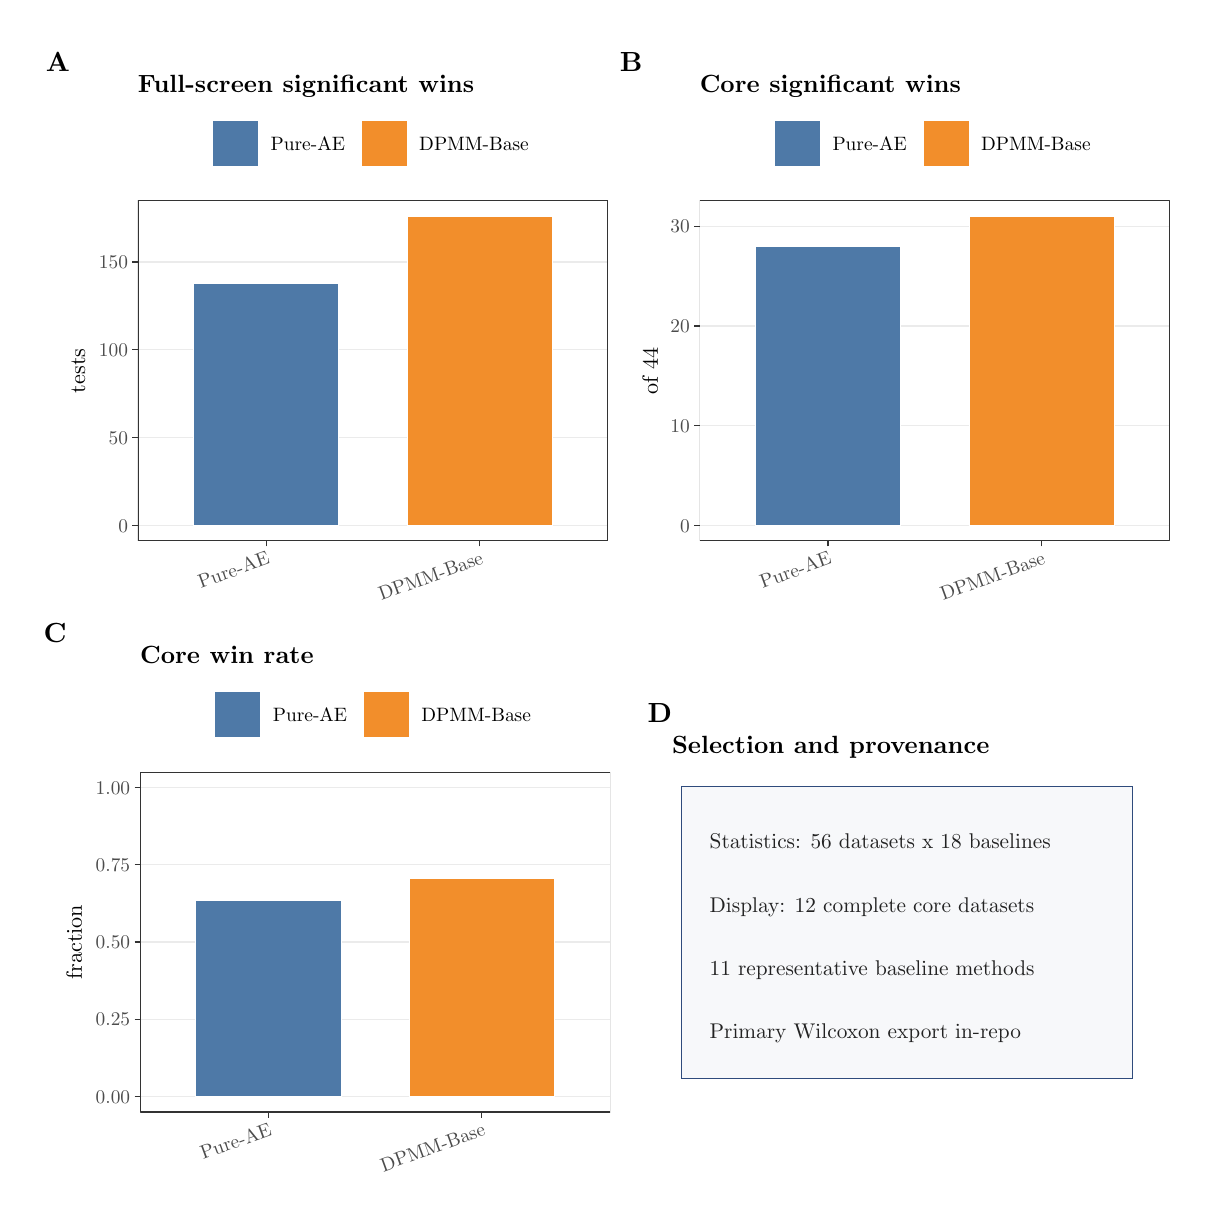
\begin{tikzpicture}[x=1pt,y=1pt]
\definecolor{fillColor}{RGB}{255,255,255}
\path[use as bounding box,fill=fillColor,fill opacity=0.00] (0,0) rectangle (421.48,423.78);
\begin{scope}
\path[clip] (  0.00,  0.00) rectangle (421.48,423.78);
\definecolor{drawColor}{RGB}{255,255,255}
\definecolor{fillColor}{RGB}{255,255,255}

\path[draw=drawColor,line width= 0.6pt,line join=round,line cap=round,fill=fillColor] (  0.00,  0.00) rectangle (421.48,423.78);
\end{scope}
\begin{scope}
\path[clip] (  5.50,211.89) rectangle (210.74,418.28);
\definecolor{drawColor}{RGB}{255,255,255}
\definecolor{fillColor}{RGB}{255,255,255}

\path[draw=drawColor,line width= 0.6pt,line join=round,line cap=round,fill=fillColor] (  5.50,211.89) rectangle (210.74,418.28);
\end{scope}
\begin{scope}
\path[clip] (210.74,211.89) rectangle (415.98,418.28);
\definecolor{drawColor}{RGB}{255,255,255}
\definecolor{fillColor}{RGB}{255,255,255}

\path[draw=drawColor,line width= 0.6pt,line join=round,line cap=round,fill=fillColor] (210.74,211.89) rectangle (415.98,418.28);
\end{scope}
\begin{scope}
\path[clip] (  4.56,212.32) rectangle (211.68,417.85);
\definecolor{drawColor}{RGB}{255,255,255}
\definecolor{fillColor}{RGB}{255,255,255}

\path[draw=drawColor,line width= 0.4pt,line join=round,line cap=round,fill=fillColor] (  4.56,212.32) rectangle (211.68,417.85);
\end{scope}
\begin{scope}
\path[clip] ( 39.85,238.34) rectangle (209.68,361.19);
\definecolor{fillColor}{RGB}{255,255,255}

\path[fill=fillColor] ( 39.85,238.34) rectangle (209.68,361.19);
\definecolor{drawColor}{gray}{0.92}

\path[draw=drawColor,line width= 0.4pt,line join=round] ( 39.85,243.92) --
	(209.68,243.92);

\path[draw=drawColor,line width= 0.4pt,line join=round] ( 39.85,275.65) --
	(209.68,275.65);

\path[draw=drawColor,line width= 0.4pt,line join=round] ( 39.85,307.38) --
	(209.68,307.38);

\path[draw=drawColor,line width= 0.4pt,line join=round] ( 39.85,339.11) --
	(209.68,339.11);
\definecolor{drawColor}{RGB}{255,255,255}
\definecolor{fillColor}{RGB}{242,142,43}

\path[draw=drawColor,line width= 0.3pt,fill=fillColor] (137.12,243.92) rectangle (189.61,355.61);
\definecolor{fillColor}{RGB}{78,121,167}

\path[draw=drawColor,line width= 0.3pt,fill=fillColor] ( 59.92,243.92) rectangle (112.41,331.49);
\definecolor{drawColor}{gray}{0.20}

\path[draw=drawColor,line width= 0.4pt,line join=round,line cap=round] ( 39.85,238.34) rectangle (209.68,361.19);
\end{scope}
\begin{scope}
\path[clip] (  0.00,  0.00) rectangle (421.48,423.78);
\definecolor{drawColor}{gray}{0.30}

\node[text=drawColor,anchor=base east,inner sep=0pt, outer sep=0pt, scale=  0.70] at ( 36.25,241.51) {0};

\node[text=drawColor,anchor=base east,inner sep=0pt, outer sep=0pt, scale=  0.70] at ( 36.25,273.24) {50};

\node[text=drawColor,anchor=base east,inner sep=0pt, outer sep=0pt, scale=  0.70] at ( 36.25,304.97) {100};

\node[text=drawColor,anchor=base east,inner sep=0pt, outer sep=0pt, scale=  0.70] at ( 36.25,336.70) {150};
\end{scope}
\begin{scope}
\path[clip] (  0.00,  0.00) rectangle (421.48,423.78);
\definecolor{drawColor}{gray}{0.20}

\path[draw=drawColor,line width= 0.4pt,line join=round] ( 37.85,243.92) --
	( 39.85,243.92);

\path[draw=drawColor,line width= 0.4pt,line join=round] ( 37.85,275.65) --
	( 39.85,275.65);

\path[draw=drawColor,line width= 0.4pt,line join=round] ( 37.85,307.38) --
	( 39.85,307.38);

\path[draw=drawColor,line width= 0.4pt,line join=round] ( 37.85,339.11) --
	( 39.85,339.11);
\end{scope}
\begin{scope}
\path[clip] (  0.00,  0.00) rectangle (421.48,423.78);
\definecolor{drawColor}{gray}{0.20}

\path[draw=drawColor,line width= 0.4pt,line join=round] ( 86.16,236.34) --
	( 86.16,238.34);

\path[draw=drawColor,line width= 0.4pt,line join=round] (163.36,236.34) --
	(163.36,238.34);
\end{scope}
\begin{scope}
\path[clip] (  0.00,  0.00) rectangle (421.48,423.78);
\definecolor{drawColor}{gray}{0.30}

\node[text=drawColor,rotate= 20.00,anchor=base east,inner sep=0pt, outer sep=0pt, scale=  0.70] at ( 87.81,230.20) {Pure-AE};

\node[text=drawColor,rotate= 20.00,anchor=base east,inner sep=0pt, outer sep=0pt, scale=  0.70] at (165.01,230.20) {DPMM-Base};
\end{scope}
\begin{scope}
\path[clip] (  0.00,  0.00) rectangle (421.48,423.78);
\definecolor{drawColor}{RGB}{0,0,0}

\node[text=drawColor,rotate= 90.00,anchor=base,inner sep=0pt, outer sep=0pt, scale=  0.80] at ( 20.76,299.76) {tests};
\end{scope}
\begin{scope}
\path[clip] (  0.00,  0.00) rectangle (421.48,423.78);
\definecolor{fillColor}{RGB}{255,255,255}

\path[fill=fillColor] ( 62.47,369.19) rectangle (187.06,394.54);
\end{scope}
\begin{scope}
\path[clip] (  0.00,  0.00) rectangle (421.48,423.78);
\definecolor{fillColor}{RGB}{255,255,255}

\path[fill=fillColor] ( 66.47,373.19) rectangle ( 83.81,390.54);
\definecolor{drawColor}{RGB}{255,255,255}
\definecolor{fillColor}{RGB}{78,121,167}

\path[draw=drawColor,line width= 0.3pt,fill=fillColor] ( 66.83,373.55) rectangle ( 83.46,390.18);
\end{scope}
\begin{scope}
\path[clip] (  0.00,  0.00) rectangle (421.48,423.78);
\definecolor{fillColor}{RGB}{255,255,255}

\path[fill=fillColor] (120.13,373.19) rectangle (137.48,390.54);
\definecolor{drawColor}{RGB}{255,255,255}
\definecolor{fillColor}{RGB}{242,142,43}

\path[draw=drawColor,line width= 0.3pt,fill=fillColor] (120.49,373.55) rectangle (137.12,390.18);
\end{scope}
\begin{scope}
\path[clip] (  0.00,  0.00) rectangle (421.48,423.78);
\definecolor{drawColor}{RGB}{0,0,0}

\node[text=drawColor,anchor=base west,inner sep=0pt, outer sep=0pt, scale=  0.70] at ( 87.81,379.46) {Pure-AE};
\end{scope}
\begin{scope}
\path[clip] (  0.00,  0.00) rectangle (421.48,423.78);
\definecolor{drawColor}{RGB}{0,0,0}

\node[text=drawColor,anchor=base west,inner sep=0pt, outer sep=0pt, scale=  0.70] at (141.48,379.46) {DPMM-Base};
\end{scope}
\begin{scope}
\path[clip] (  0.00,  0.00) rectangle (421.48,423.78);
\definecolor{drawColor}{RGB}{0,0,0}

\node[text=drawColor,anchor=base west,inner sep=0pt, outer sep=0pt, scale=  0.90] at ( 39.85,400.53) {\bfseries Full-screen significant wins};
\end{scope}
\begin{scope}
\path[clip] (  0.00,  0.00) rectangle (421.48,423.78);
\definecolor{drawColor}{RGB}{0,0,0}

\node[text=drawColor,anchor=base,inner sep=0pt, outer sep=0pt, scale=  1.00] at ( 10.90,407.84) {\bfseries A};
\end{scope}
\begin{scope}
\path[clip] (212.01,212.32) rectangle (414.71,417.85);
\definecolor{drawColor}{RGB}{255,255,255}
\definecolor{fillColor}{RGB}{255,255,255}

\path[draw=drawColor,line width= 0.4pt,line join=round,line cap=round,fill=fillColor] (212.01,212.32) rectangle (414.71,417.85);
\end{scope}
\begin{scope}
\path[clip] (242.87,238.34) rectangle (412.71,361.19);
\definecolor{fillColor}{RGB}{255,255,255}

\path[fill=fillColor] (242.87,238.34) rectangle (412.71,361.19);
\definecolor{drawColor}{gray}{0.92}

\path[draw=drawColor,line width= 0.4pt,line join=round] (242.87,243.92) --
	(412.71,243.92);

\path[draw=drawColor,line width= 0.4pt,line join=round] (242.87,279.95) --
	(412.71,279.95);

\path[draw=drawColor,line width= 0.4pt,line join=round] (242.87,315.98) --
	(412.71,315.98);

\path[draw=drawColor,line width= 0.4pt,line join=round] (242.87,352.01) --
	(412.71,352.01);
\definecolor{drawColor}{RGB}{255,255,255}
\definecolor{fillColor}{RGB}{242,142,43}

\path[draw=drawColor,line width= 0.3pt,fill=fillColor] (340.14,243.92) rectangle (392.64,355.61);
\definecolor{fillColor}{RGB}{78,121,167}

\path[draw=drawColor,line width= 0.3pt,fill=fillColor] (262.95,243.92) rectangle (315.44,344.80);
\definecolor{drawColor}{gray}{0.20}

\path[draw=drawColor,line width= 0.4pt,line join=round,line cap=round] (242.87,238.34) rectangle (412.71,361.19);
\end{scope}
\begin{scope}
\path[clip] (  0.00,  0.00) rectangle (421.48,423.78);
\definecolor{drawColor}{gray}{0.30}

\node[text=drawColor,anchor=base east,inner sep=0pt, outer sep=0pt, scale=  0.70] at (239.27,241.51) {0};

\node[text=drawColor,anchor=base east,inner sep=0pt, outer sep=0pt, scale=  0.70] at (239.27,277.54) {10};

\node[text=drawColor,anchor=base east,inner sep=0pt, outer sep=0pt, scale=  0.70] at (239.27,313.57) {20};

\node[text=drawColor,anchor=base east,inner sep=0pt, outer sep=0pt, scale=  0.70] at (239.27,349.60) {30};
\end{scope}
\begin{scope}
\path[clip] (  0.00,  0.00) rectangle (421.48,423.78);
\definecolor{drawColor}{gray}{0.20}

\path[draw=drawColor,line width= 0.4pt,line join=round] (240.87,243.92) --
	(242.87,243.92);

\path[draw=drawColor,line width= 0.4pt,line join=round] (240.87,279.95) --
	(242.87,279.95);

\path[draw=drawColor,line width= 0.4pt,line join=round] (240.87,315.98) --
	(242.87,315.98);

\path[draw=drawColor,line width= 0.4pt,line join=round] (240.87,352.01) --
	(242.87,352.01);
\end{scope}
\begin{scope}
\path[clip] (  0.00,  0.00) rectangle (421.48,423.78);
\definecolor{drawColor}{gray}{0.20}

\path[draw=drawColor,line width= 0.4pt,line join=round] (289.19,236.34) --
	(289.19,238.34);

\path[draw=drawColor,line width= 0.4pt,line join=round] (366.39,236.34) --
	(366.39,238.34);
\end{scope}
\begin{scope}
\path[clip] (  0.00,  0.00) rectangle (421.48,423.78);
\definecolor{drawColor}{gray}{0.30}

\node[text=drawColor,rotate= 20.00,anchor=base east,inner sep=0pt, outer sep=0pt, scale=  0.70] at (290.84,230.20) {Pure-AE};

\node[text=drawColor,rotate= 20.00,anchor=base east,inner sep=0pt, outer sep=0pt, scale=  0.70] at (368.04,230.20) {DPMM-Base};
\end{scope}
\begin{scope}
\path[clip] (  0.00,  0.00) rectangle (421.48,423.78);
\definecolor{drawColor}{RGB}{0,0,0}

\node[text=drawColor,rotate= 90.00,anchor=base,inner sep=0pt, outer sep=0pt, scale=  0.80] at (227.69,299.76) {of 44};
\end{scope}
\begin{scope}
\path[clip] (  0.00,  0.00) rectangle (421.48,423.78);
\definecolor{fillColor}{RGB}{255,255,255}

\path[fill=fillColor] (265.50,369.19) rectangle (390.09,394.54);
\end{scope}
\begin{scope}
\path[clip] (  0.00,  0.00) rectangle (421.48,423.78);
\definecolor{fillColor}{RGB}{255,255,255}

\path[fill=fillColor] (269.50,373.19) rectangle (286.84,390.54);
\definecolor{drawColor}{RGB}{255,255,255}
\definecolor{fillColor}{RGB}{78,121,167}

\path[draw=drawColor,line width= 0.3pt,fill=fillColor] (269.85,373.55) rectangle (286.49,390.18);
\end{scope}
\begin{scope}
\path[clip] (  0.00,  0.00) rectangle (421.48,423.78);
\definecolor{fillColor}{RGB}{255,255,255}

\path[fill=fillColor] (323.16,373.19) rectangle (340.50,390.54);
\definecolor{drawColor}{RGB}{255,255,255}
\definecolor{fillColor}{RGB}{242,142,43}

\path[draw=drawColor,line width= 0.3pt,fill=fillColor] (323.51,373.55) rectangle (340.15,390.18);
\end{scope}
\begin{scope}
\path[clip] (  0.00,  0.00) rectangle (421.48,423.78);
\definecolor{drawColor}{RGB}{0,0,0}

\node[text=drawColor,anchor=base west,inner sep=0pt, outer sep=0pt, scale=  0.70] at (290.84,379.46) {Pure-AE};
\end{scope}
\begin{scope}
\path[clip] (  0.00,  0.00) rectangle (421.48,423.78);
\definecolor{drawColor}{RGB}{0,0,0}

\node[text=drawColor,anchor=base west,inner sep=0pt, outer sep=0pt, scale=  0.70] at (344.50,379.46) {DPMM-Base};
\end{scope}
\begin{scope}
\path[clip] (  0.00,  0.00) rectangle (421.48,423.78);
\definecolor{drawColor}{RGB}{0,0,0}

\node[text=drawColor,anchor=base west,inner sep=0pt, outer sep=0pt, scale=  0.90] at (242.87,400.53) {\bfseries Core significant wins};
\end{scope}
\begin{scope}
\path[clip] (  0.00,  0.00) rectangle (421.48,423.78);
\definecolor{drawColor}{RGB}{0,0,0}

\node[text=drawColor,anchor=base,inner sep=0pt, outer sep=0pt, scale=  1.00] at (218.10,407.84) {\bfseries B};
\end{scope}
\begin{scope}
\path[clip] (  5.50,  5.50) rectangle (210.74,211.89);
\definecolor{drawColor}{RGB}{255,255,255}
\definecolor{fillColor}{RGB}{255,255,255}

\path[draw=drawColor,line width= 0.6pt,line join=round,line cap=round,fill=fillColor] (  5.50,  5.50) rectangle (210.74,211.89);
\end{scope}
\begin{scope}
\path[clip] (210.74,  5.50) rectangle (415.98,211.89);
\definecolor{drawColor}{RGB}{255,255,255}
\definecolor{fillColor}{RGB}{255,255,255}

\path[draw=drawColor,line width= 0.6pt,line join=round,line cap=round,fill=fillColor] (210.74,  5.50) rectangle (415.98,211.89);
\end{scope}
\begin{scope}
\path[clip] (  3.78,  5.93) rectangle (212.46,211.46);
\definecolor{drawColor}{RGB}{255,255,255}
\definecolor{fillColor}{RGB}{255,255,255}

\path[draw=drawColor,line width= 0.4pt,line join=round,line cap=round,fill=fillColor] (  3.78,  5.93) rectangle (212.46,211.46);
\end{scope}
\begin{scope}
\path[clip] ( 40.63, 31.95) rectangle (210.46,154.81);
\definecolor{fillColor}{RGB}{255,255,255}

\path[fill=fillColor] ( 40.63, 31.95) rectangle (210.46,154.81);
\definecolor{drawColor}{gray}{0.92}

\path[draw=drawColor,line width= 0.4pt,line join=round] ( 40.63, 37.53) --
	(210.46, 37.53);

\path[draw=drawColor,line width= 0.4pt,line join=round] ( 40.63, 65.45) --
	(210.46, 65.45);

\path[draw=drawColor,line width= 0.4pt,line join=round] ( 40.63, 93.38) --
	(210.46, 93.38);

\path[draw=drawColor,line width= 0.4pt,line join=round] ( 40.63,121.30) --
	(210.46,121.30);

\path[draw=drawColor,line width= 0.4pt,line join=round] ( 40.63,149.22) --
	(210.46,149.22);
\definecolor{drawColor}{RGB}{255,255,255}
\definecolor{fillColor}{RGB}{242,142,43}

\path[draw=drawColor,line width= 0.3pt,fill=fillColor] (137.90, 37.53) rectangle (190.39,116.27);
\definecolor{fillColor}{RGB}{78,121,167}

\path[draw=drawColor,line width= 0.3pt,fill=fillColor] ( 60.70, 37.53) rectangle (113.19,108.57);
\definecolor{drawColor}{gray}{0.20}

\path[draw=drawColor,line width= 0.4pt,line join=round,line cap=round] ( 40.63, 31.95) rectangle (210.46,154.81);
\end{scope}
\begin{scope}
\path[clip] (  0.00,  0.00) rectangle (421.48,423.78);
\definecolor{drawColor}{gray}{0.30}

\node[text=drawColor,anchor=base east,inner sep=0pt, outer sep=0pt, scale=  0.70] at ( 37.03, 35.12) {0.00};

\node[text=drawColor,anchor=base east,inner sep=0pt, outer sep=0pt, scale=  0.70] at ( 37.03, 63.04) {0.25};

\node[text=drawColor,anchor=base east,inner sep=0pt, outer sep=0pt, scale=  0.70] at ( 37.03, 90.97) {0.50};

\node[text=drawColor,anchor=base east,inner sep=0pt, outer sep=0pt, scale=  0.70] at ( 37.03,118.89) {0.75};

\node[text=drawColor,anchor=base east,inner sep=0pt, outer sep=0pt, scale=  0.70] at ( 37.03,146.81) {1.00};
\end{scope}
\begin{scope}
\path[clip] (  0.00,  0.00) rectangle (421.48,423.78);
\definecolor{drawColor}{gray}{0.20}

\path[draw=drawColor,line width= 0.4pt,line join=round] ( 38.63, 37.53) --
	( 40.63, 37.53);

\path[draw=drawColor,line width= 0.4pt,line join=round] ( 38.63, 65.45) --
	( 40.63, 65.45);

\path[draw=drawColor,line width= 0.4pt,line join=round] ( 38.63, 93.38) --
	( 40.63, 93.38);

\path[draw=drawColor,line width= 0.4pt,line join=round] ( 38.63,121.30) --
	( 40.63,121.30);

\path[draw=drawColor,line width= 0.4pt,line join=round] ( 38.63,149.22) --
	( 40.63,149.22);
\end{scope}
\begin{scope}
\path[clip] (  0.00,  0.00) rectangle (421.48,423.78);
\definecolor{drawColor}{gray}{0.20}

\path[draw=drawColor,line width= 0.4pt,line join=round] ( 86.95, 29.95) --
	( 86.95, 31.95);

\path[draw=drawColor,line width= 0.4pt,line join=round] (164.14, 29.95) --
	(164.14, 31.95);
\end{scope}
\begin{scope}
\path[clip] (  0.00,  0.00) rectangle (421.48,423.78);
\definecolor{drawColor}{gray}{0.30}

\node[text=drawColor,rotate= 20.00,anchor=base east,inner sep=0pt, outer sep=0pt, scale=  0.70] at ( 88.60, 23.82) {Pure-AE};

\node[text=drawColor,rotate= 20.00,anchor=base east,inner sep=0pt, outer sep=0pt, scale=  0.70] at (165.79, 23.82) {DPMM-Base};
\end{scope}
\begin{scope}
\path[clip] (  0.00,  0.00) rectangle (421.48,423.78);
\definecolor{drawColor}{RGB}{0,0,0}

\node[text=drawColor,rotate= 90.00,anchor=base,inner sep=0pt, outer sep=0pt, scale=  0.80] at ( 19.59, 93.38) {fraction};
\end{scope}
\begin{scope}
\path[clip] (  0.00,  0.00) rectangle (421.48,423.78);
\definecolor{fillColor}{RGB}{255,255,255}

\path[fill=fillColor] ( 63.25,162.81) rectangle (187.84,188.15);
\end{scope}
\begin{scope}
\path[clip] (  0.00,  0.00) rectangle (421.48,423.78);
\definecolor{fillColor}{RGB}{255,255,255}

\path[fill=fillColor] ( 67.25,166.81) rectangle ( 84.60,184.15);
\definecolor{drawColor}{RGB}{255,255,255}
\definecolor{fillColor}{RGB}{78,121,167}

\path[draw=drawColor,line width= 0.3pt,fill=fillColor] ( 67.61,167.16) rectangle ( 84.24,183.79);
\end{scope}
\begin{scope}
\path[clip] (  0.00,  0.00) rectangle (421.48,423.78);
\definecolor{fillColor}{RGB}{255,255,255}

\path[fill=fillColor] (120.91,166.81) rectangle (138.26,184.15);
\definecolor{drawColor}{RGB}{255,255,255}
\definecolor{fillColor}{RGB}{242,142,43}

\path[draw=drawColor,line width= 0.3pt,fill=fillColor] (121.27,167.16) rectangle (137.90,183.79);
\end{scope}
\begin{scope}
\path[clip] (  0.00,  0.00) rectangle (421.48,423.78);
\definecolor{drawColor}{RGB}{0,0,0}

\node[text=drawColor,anchor=base west,inner sep=0pt, outer sep=0pt, scale=  0.70] at ( 88.60,173.07) {Pure-AE};
\end{scope}
\begin{scope}
\path[clip] (  0.00,  0.00) rectangle (421.48,423.78);
\definecolor{drawColor}{RGB}{0,0,0}

\node[text=drawColor,anchor=base west,inner sep=0pt, outer sep=0pt, scale=  0.70] at (142.26,173.07) {DPMM-Base};
\end{scope}
\begin{scope}
\path[clip] (  0.00,  0.00) rectangle (421.48,423.78);
\definecolor{drawColor}{RGB}{0,0,0}

\node[text=drawColor,anchor=base west,inner sep=0pt, outer sep=0pt, scale=  0.90] at ( 40.63,194.14) {\bfseries Core win rate};
\end{scope}
\begin{scope}
\path[clip] (  0.00,  0.00) rectangle (421.48,423.78);
\definecolor{drawColor}{RGB}{0,0,0}

\node[text=drawColor,anchor=base,inner sep=0pt, outer sep=0pt, scale=  1.00] at (  9.93,201.45) {\bfseries C};
\end{scope}
\begin{scope}
\path[clip] (222.03, 34.61) rectangle (404.68,182.78);

\path[] (222.03, 34.61) rectangle (404.68,182.78);
\end{scope}
\begin{scope}
\path[clip] (232.85, 36.61) rectangle (402.68,159.47);
\definecolor{drawColor}{RGB}{47,75,124}
\definecolor{fillColor}{RGB}{247,248,250}

\path[draw=drawColor,line width= 0.5pt,fill=fillColor] (236.25, 43.98) rectangle (399.29,149.64);
\definecolor{drawColor}{RGB}{34,34,34}

\node[text=drawColor,anchor=base west,inner sep=0pt, outer sep=0pt, scale=  0.77] at (246.44,127.15) {Statistics: 56 datasets x 18 baselines};

\node[text=drawColor,anchor=base west,inner sep=0pt, outer sep=0pt, scale=  0.77] at (246.44,104.22) {Display: 12 complete core datasets};

\node[text=drawColor,anchor=base west,inner sep=0pt, outer sep=0pt, scale=  0.77] at (246.44, 81.28) {11 representative baseline methods};

\node[text=drawColor,anchor=base west,inner sep=0pt, outer sep=0pt, scale=  0.77] at (246.44, 58.35) {Primary Wilcoxon export in-repo};
\end{scope}
\begin{scope}
\path[clip] (  0.00,  0.00) rectangle (421.48,423.78);
\definecolor{drawColor}{RGB}{0,0,0}

\node[text=drawColor,anchor=base west,inner sep=0pt, outer sep=0pt, scale=  0.90] at (232.85,161.46) {\bfseries Selection and provenance};
\end{scope}
\begin{scope}
\path[clip] (  0.00,  0.00) rectangle (421.48,423.78);
\definecolor{drawColor}{RGB}{0,0,0}

\node[text=drawColor,anchor=base,inner sep=0pt, outer sep=0pt, scale=  1.00] at (228.44,172.77) {\bfseries D};
\end{scope}
\end{tikzpicture}
